% Template for a Computer Science Tripos Part II project dissertation
\documentclass[12pt,a4paper,twoside,openright]{report}
\usepackage[pdfborder={0 0 0}]{hyperref}    % turns references into hyperlinks
\usepackage[margin=25mm]{geometry}  % adjusts page layout
\usepackage{graphicx}  % allows inclusion of PDF, PNG and JPG images
\usepackage{verbatim}
\usepackage{docmute}   % only needed to allow inclusion of proposal.tex

\raggedbottom                           % try to avoid widows and orphans
\sloppy
\clubpenalty1000%
\widowpenalty1000%

\renewcommand{\baselinestretch}{1.1}    % adjust line spacing to make
                                        % more readable

\begin{document}

\bibliographystyle{plain}


%%%%%%%%%%%%%%%%%%%%%%%%%%%%%%%%%%%%%%%%%%%%%%%%%%%%%%%%%%%%%%%%%%%%%%%%
% Title


\pagestyle{empty}

\rightline{\LARGE \textbf{Martin Richards}}

\vspace*{60mm}
\begin{center}
\Huge
\textbf{How to write a dissertation in \LaTeX} \\[5mm]
Computer Science Tripos -- Part II \\[5mm]
St John's College \\[5mm]
\today  % today's date
\end{center}

%%%%%%%%%%%%%%%%%%%%%%%%%%%%%%%%%%%%%%%%%%%%%%%%%%%%%%%%%%%%%%%%%%%%%%%%%%%%%%
% Proforma, table of contents and list of figures

\pagestyle{plain}

\chapter*{Proforma}

{\large
\begin{tabular}{ll}
Name:               & \bf Martin Richards                       \\
College:            & \bf St John's College                     \\
Project Title:      & \bf How to write a dissertation in \LaTeX \\
Examination:        & \bf Computer Science Tripos -- Part II, July 2001  \\
Word Count:         & \bf 1587\footnotemark[1]
                      (well less than the 12000 limit)  \\
Project Originator: & Dr M.~Richards                    \\
Supervisor:         & Dr Markus Kuhn                    \\ 
\end{tabular}
}
\footnotetext[1]{This word count was computed
by \texttt{detex diss.tex | tr -cd '0-9A-Za-z $\tt\backslash$n' | wc -w}
}
\stepcounter{footnote}


\section*{Original Aims of the Project}

To write a demonstration dissertation\footnote{A normal footnote without the
complication of being in a table.} using \LaTeX\ to save
student's time when writing their own dissertations. The dissertation
should illustrate how to use the more common \LaTeX\ constructs. It
should include pictures and diagrams to show how these can be
incorporated into the dissertation.  It should contain the entire
\LaTeX\ source of the dissertation and the makefile.  It should
explain how to construct an MSDOS disk of the dissertation in
Postscript format that can be used by the book shop for printing, and,
finally, it should have the prescribed layout and format of a diploma
dissertation.


\section*{Work Completed}

All that has been completed appears in this dissertation.

\section*{Special Difficulties}

Learning how to incorporate encapulated postscript into a \LaTeX\
document on both Ubuntu Linux and OS X.
 
\newpage
\section*{Declaration}

I, [Name] of [College], being a candidate for Part II of the Computer
Science Tripos [or the Diploma in Computer Science], hereby declare
that this dissertation and the work described in it are my own work,
unaided except as may be specified below, and that the dissertation
does not contain material that has already been used to any substantial
extent for a comparable purpose.

\bigskip
\leftline{Signed [signature]}

\medskip
\leftline{Date [date]}

\tableofcontents

\listoffigures

\newpage
\section*{Acknowledgements}

This document owes much to an earlier version written by Simon Moore
\cite{Moore95}.  His help, encouragement and advice was greatly 
appreciated.

%%%%%%%%%%%%%%%%%%%%%%%%%%%%%%%%%%%%%%%%%%%%%%%%%%%%%%%%%%%%%%%%%%%%%%%
% now for the chapters

\pagestyle{headings}

\chapter{Introduction}

\section{Overview of the files}

This document consists of the following files:

\begin{itemize}
\item \texttt{makefile} --- The makefile for the dissertation and
                         Project Proposal
\item \texttt{diss.tex} --- The dissertation
\item \texttt{proposal.tex}  --- The project proposal 
\item \texttt{figs} -- A directory containing diagrams and pictures
\item \texttt{refs.bib} --- The bibliography database
\end{itemize}

\section{Building the document}

This document was produced using \LaTeXe which is based upon
\LaTeX\cite{Lamport86}.  To build the document you first need to
generate \texttt{diss.aux} which, amongst other things, contains the
references used.  This if done by executing the command:

\texttt{pdflatex diss}

\noindent
Then the bibliography can be generated from \texttt{refs.bib} using:

\texttt{bibtex diss}

\noindent
Finally, to ensure all the page numbering is correct run \texttt{pdflatex}
on \texttt{diss.tex} until the \texttt{.aux} files do not change.  This
usually takes 2 more runs.

\subsection{The makefile}

To simplify the calls to \texttt{pdflatex} and \texttt{bibtex}, 
a makefile has been provided, see Appendix~\ref{makefile}. 
It provides the following facilities:

\begin{description}

\item\texttt{make} \\
 Display help information.

\item\texttt{make proposal.pdf} \\
 Format the proposal document as a PDF.

\item\texttt{make view-proposal} \\
 Run \texttt{make proposal.pdf} and then display it with a Linux PDF viewer
 (preferably ``okular'', if that is not available fall back to ``evince'').

\item\texttt{make diss.pdf} \\
 Format the dissertation document as a PDF.

\item\texttt{make count} \\
Display an estimate of the word count.

\item\texttt{make all} \\
Construct \texttt{proposal.pdf} and \texttt{diss.pdf}.

\item\texttt{make pub} \\ Make \texttt{diss.pdf}
and place it in my \texttt{public\_html} directory.

\item\texttt{make clean} \\ Delete all intermediate files except the
source files and the resulting PDFs. All these deleted files can
be reconstructed by typing \texttt{make all}.

\end{description}


\section{Counting words}

An approximate word count of the body of the dissertation may be
obtained using:

\texttt{wc diss.tex}

\noindent
Alternatively, try something like:

\verb/detex diss.tex | tr -cd '0-9A-Z a-z\n' | wc -w/


\chapter{Preparation}

This chapter is empty!


\chapter{Implementation}

\section{Verbatim text}

Verbatim text can be included using \verb|\begin{verbatim}| and
\verb|\end{verbatim}|. I normally use a slightly smaller font and
often squeeze the lines a little closer together, as in:

{\renewcommand{\baselinestretch}{0.8}\small
\begin{verbatim}
GET "libhdr"
 
GLOBAL { count:200; all  }
 
LET try(ld, row, rd) BE TEST row=all
                        THEN count := count + 1
                        ELSE { LET poss = all & ~(ld | row | rd)
                               UNTIL poss=0 DO
                               { LET p = poss & -poss
                                 poss := poss - p
                                 try(ld+p << 1, row+p, rd+p >> 1)
                               }
                             }
LET start() = VALOF
{ all := 1
  FOR i = 1 TO 12 DO
  { count := 0
    try(0, 0, 0)
    writef("Number of solutions to %i2-queens is %i5*n", i, count)
    all := 2*all + 1
  }
  RESULTIS 0
}
\end{verbatim}
}

\section{Tables}

\begin{samepage}
Here is a simple example\footnote{A footnote} of a table.

\begin{center}
\begin{tabular}{l|c|r}
Left      & Centred & Right \\
Justified &         & Justified \\[3mm]
%\hline\\%[-2mm]
First     & A       & XXX \\
Second    & AA      & XX  \\
Last      & AAA     & X   \\
\end{tabular}
\end{center}

\noindent
There is another example table in the proforma.
\end{samepage}

\section{Simple diagrams}

Simple diagrams can be written directly in \LaTeX.  For example, see
figure~\ref{latexpic1} on page~\pageref{latexpic1} and see
figure~\ref{latexpic2} on page~\pageref{latexpic2}.

\begin{figure}
\setlength{\unitlength}{1mm}
\begin{center}
\begin{picture}(125,100)
\put(0,80){\framebox(50,10){AAA}}
\put(0,60){\framebox(50,10){BBB}}
\put(0,40){\framebox(50,10){CCC}}
\put(0,20){\framebox(50,10){DDD}}
\put(0,00){\framebox(50,10){EEE}}

\put(75,80){\framebox(50,10){XXX}}
\put(75,60){\framebox(50,10){YYY}}
\put(75,40){\framebox(50,10){ZZZ}}

\put(25,80){\vector(0,-1){10}}
\put(25,60){\vector(0,-1){10}}
\put(25,50){\vector(0,1){10}}
\put(25,40){\vector(0,-1){10}}
\put(25,20){\vector(0,-1){10}}

\put(100,80){\vector(0,-1){10}}
\put(100,70){\vector(0,1){10}}
\put(100,60){\vector(0,-1){10}}
\put(100,50){\vector(0,1){10}}

\put(50,65){\vector(1,0){25}}
\put(75,65){\vector(-1,0){25}}
\end{picture}
\end{center}
\caption{A picture composed of boxes and vectors.}
\label{latexpic1}
\end{figure}

\begin{figure}
\setlength{\unitlength}{1mm}
\begin{center}

\begin{picture}(100,70)
\put(47,65){\circle{10}}
\put(45,64){abc}

\put(37,45){\circle{10}}
\put(37,51){\line(1,1){7}}
\put(35,44){def}

\put(57,25){\circle{10}}
\put(57,31){\line(-1,3){9}}
\put(57,31){\line(-3,2){15}}
\put(55,24){ghi}

\put(32,0){\framebox(10,10){A}}
\put(52,0){\framebox(10,10){B}}
\put(37,12){\line(0,1){26}}
\put(37,12){\line(2,1){15}}
\put(57,12){\line(0,2){6}}
\end{picture}

\end{center}
\caption{A diagram composed of circles, lines and boxes.}
\label{latexpic2}
\end{figure}



\section{Adding more complicated graphics}

The use of \LaTeX\ format can be tedious and it is often better to use
encapsulated postscript (EPS) or PDF to represent complicated graphics.
Figure~\ref{epsfig} and~\ref{xfig} on page \pageref{xfig} are
examples. The second figure was drawn using \texttt{xfig} and exported in
{\tt.eps} format. This is my recommended way of drawing all diagrams.


\begin{figure}[tbh]
\centerline{
\includegraphics{figs/cuarms.pdf}}
\caption{Example figure using encapsulated postscript}
\label{epsfig}
\end{figure}

\begin{figure}[tbh]
\vspace{4in}
\caption{Example figure where a picture can be pasted in}
\label{pastedfig}
\end{figure}


\begin{figure}[tbh]
\centerline{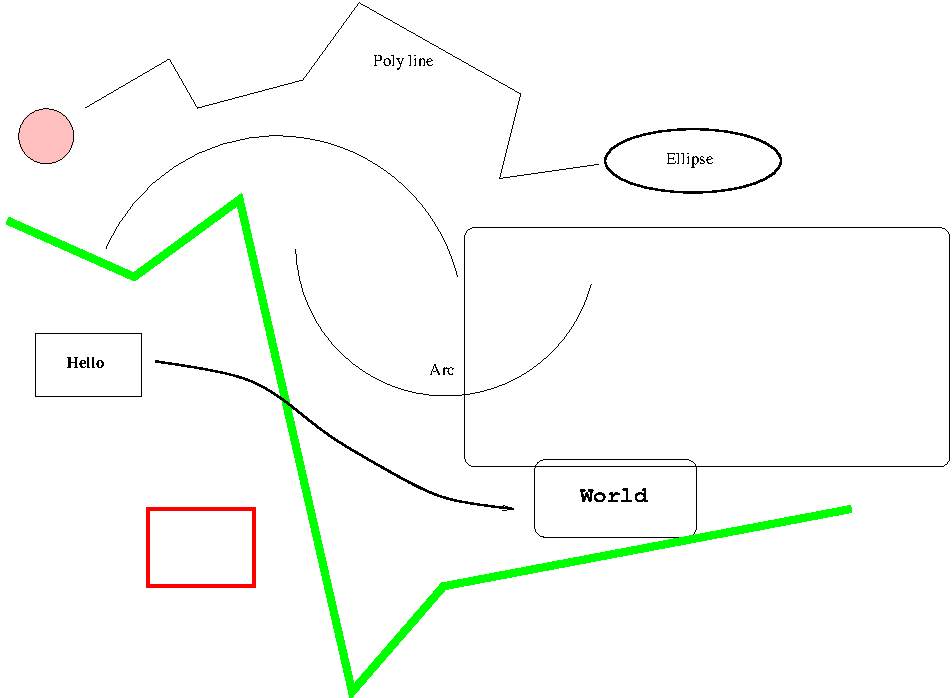
\includegraphics{figs/diagram.pdf}}
\caption{Example diagram drawn using \texttt{xfig}}
\label{xfig}
\end{figure}


\chapter{Evaluation}

\section{Printing and binding}

Use a ``duplex'' laser printer that can print on both sides to print
two copies of your dissertation. Then bind them, for example using the
comb binder in the Computer Laboratory Library.

\section{Further information}

See the Unix Tools notes at

\url{http://www.cl.cam.ac.uk/teaching/current-1/UnixTools/materials.html}


\chapter{Conclusion}

I hope that this rough guide to writing a dissertation is \LaTeX\ has
been helpful and saved you time.


%%%%%%%%%%%%%%%%%%%%%%%%%%%%%%%%%%%%%%%%%%%%%%%%%%%%%%%%%%%%%%%%%%%%%
% the bibliography
\addcontentsline{toc}{chapter}{Bibliography}
\bibliography{refs}

%%%%%%%%%%%%%%%%%%%%%%%%%%%%%%%%%%%%%%%%%%%%%%%%%%%%%%%%%%%%%%%%%%%%%
% the appendices
\appendix

\chapter{Latex source}

\section{diss.tex}
{\scriptsize\verbatiminput{diss.tex}}

\section{proposal.tex}
{\scriptsize\verbatiminput{proposal.tex}}

\chapter{Makefile}

\section{makefile}\label{makefile}
{\scriptsize\verbatiminput{makefile.txt}}

\section{refs.bib}
{\scriptsize\verbatiminput{refs.bib}}


\chapter{Project Proposal}

% Note: this file can be compiled on its own, but is also included by
% diss.tex (using the docmute.sty package to ignore the preamble)
\documentclass[12pt,a4paper,twoside]{article}
\usepackage[pdfborder={0 0 0}]{hyperref}
\usepackage[margin=25mm]{geometry}
\usepackage{graphicx}
\begin{document}

\vfil

\centerline{\Large Computer Science Project Proposal}
\vspace{0.4in}
\centerline{\Large Path ORAM on MirageOS}
\vspace{0.4in}
\centerline{\large R. Horlick, Homerton College}
\vspace{0.3in}
\centerline{\large Originator: Dr N. Sultana}
\vspace{0.3in}
\centerline{\large 15 October 2015}

\vfil


\noindent
{\bf Project Supervisors:} Dr N. Sultana \& Dr R. M. Mortier
\vspace{0.2in}

\noindent
{\bf Director of Studies:} Dr B. Roman
\vspace{0.2in}
\noindent
 
\noindent
{\bf Project Overseers:} Dr M. G. Kuhn \& Prof P. E. Sewell


% Main document

\section*{Introduction and Description of the Work}

As the cost of large-scale cloud storage decreases and the rate of data production grows, individuals and small businesses will find themselves increasing reliant on the trust of cloud providers. We can, of course, use encryption and be safe in the knowledge that no adversary will be able to view the plaintext of our data, but this is not enough. It turns out that the pattern of access to the data can leak large amounts of information. In a study on an encrypted email repository, up to 80\% of search queries could be inferred from the access pattern alone! So clearly this a leak worth plugging, but how can we do it?

The solution to our problem is Oblivious Random Access Memory (ORAM), a cryptographic primitive that ensures that an adversary has negligible probability of learning anything about the logical access pattern, even with full access to the physical one. We normally talk about an ORAM as a block device, with $N$ blocks of $B$ bits each, giving an ORAM of size $N \cdot B$. We are most interested in the asymptotic bandwidth cost of the ORAM protocol, because we are operating over the internet.

A trivial ORAM algorithm operates by scanning over the whole ORAM and reading/updating only the relevant block, but this has $O(N)$ bandwidth cost, which is highly impractical for large-scale storage. Luckily, much better algorithms have been proposed. We choose to focus on Path ORAM, because it has only $O(\log N)$ bandwidth cost in the worst case if $B = \Omega(\log^2 N)$, as well as being incredibly simple conceptually.

ORAM protocols generally operate in a client-server model. For our purposes the server is the cloud storage provider and the client will be a MirageOS cloud instance. MirageOS is a unikernel operating system designed to run on the Xen hypervisor. I have chosen to use Mirage for a number of reasons. Firstly, it is lightweight and designed to be run in the cloud, meaning that simple cloud services can be built on top of it that fully leverage the ORAM. Secondly, it is written in OCaml, meaning that I can take full advantage of the rich module system. This will allow me to write my implementation as a functor that takes an implementation of Mirage's BLOCK interface and creates a new BLOCK implementation that uses ORAM, as shown in Figure \ref{miragestack}. This means that the ORAM could be used with any underlying implementation of the BLOCK interface and that it would plug seamlessly into any existing program.

\begin{figure}
\setlength{\unitlength}{0.75mm}
\begin{center}
\begin{picture}(155,60)
\put(0,30){\framebox(50,10){External Storage}}
\put(0,20){\framebox(50,10){BLOCK}}
\put(25,10){\vector(0,1){10}}
\put(25,20){\vector(0,-1){10}}
\put(56,13.2){BLOCK Interface}
\multiput(0,15)(4,0){14}{\line(1,0){2}}
\multiput(101,15)(4,0){14}{\line(1,0){2}}
\put(56,33.2){BLOCK Interface}
\multiput(101,35)(4,0){14}{\line(1,0){2}}
\put(0,00){\framebox(50,10){MirageOS}}

\put(105,50){\framebox(50,10){External Storage}}
\put(105,40){\framebox(50,10){BLOCK}}
\put(130,30){\vector(0,1){10}}
\put(130,40){\vector(0,-1){10}}
\put(105,20){\framebox(50,10){ORAM}}
\put(130,10){\vector(0,1){10}}
\put(130,20){\vector(0,-1){10}}
\put(105,00){\framebox(50,10){MirageOS}}
\end{picture}
\end{center}
\caption{The MirageOS stack with and without ORAM}
\label{miragestack}
\end{figure}

\section*{Starting Point}

MirageOS is a framework, that pulls together a number of libraries and syntax extensions, to provide a lightweight unikernel operating system. It provides a command line tool for generating the main file, that links together implementations of various parts of the system, and passes them to the unikernel. There are a number of module signatures that define the operation of devices, such as CONSOLE for consoles, ETHIF for ethernet, and most importantly for us BLOCK, for block devices.

There are currently two implementations of the BLOCK interface, one for Unix and one for Xen, and I would like to support both. Thus I will build a functor that takes one of these and emulates a block device using it, adding ORAM to it. This will most likely use some of the algorithms/code from the existing implementations, for dealing with buffers, implemented using the Cstruct library.

\section*{Substance and Structure of the Project}

\subsection*{Substance}

The Path ORAM protocol has three main components: a binary tree, a stash and a position map. The binary tree is the main storage space. Every node in the tree is a bucket, which can contain up to $Z$ blocks. The tree has height $L$, where the tree of height 0 consists only of the root node, and the leaves are at level $L$. The stash is temporary client-side storage, consisting only of a set of blocks waiting to be put back into the tree. The position map associates, with each block ID, an integer between 0 and $2^L-1$. The invariant that the Path ORAM algorithm maintains is that if the position of a block $x$ is $p$, then $x$ is either in some bucket along the path from the root node to the $p^{th}$ leaf, or in the stash. On every access to the tree, a whole path is read into, the accessed block is assigned a new random position and then as many blocks as possible are written back into the same path. This means that in any two access to the same block, the paths that are read are statistically independent.

We can extend the basic path ORAM algorithm with recursion. That is, calling the data ORAM $ORAM_0$, we store the position map of $ORAM_0$ in a smaller ORAM, $ORAM_1$, and the position map for this in an even smaller ORAM, $ORAM_2$. We can do this until we have a sufficiently small position map on the client. Supposing that we store $\chi$ leaf addresses in each PosMap ORAM, the position for a data block with address $a_0$ is at $a_1 = a_0 / \chi$ in $ORAM_1$, and in general $a_n = a_0 / \chi^n$ for the address in $ORAM_n$. 

Recursion does add an overhead, but we can reduce this overhead by exploiting locality. Assuming that programs will access adjacent data blocks, we can cache PosMap blocks in a PosMap Lookaside Buffer, so that if all $\chi$ data blocks that are referenced in a PosMap block are accessed in turn we only need to do the recursion once. Doing this na\"ively, however, breaks security, because we are revealing information through the cache hit pattern. To avoid this we use Unified ORAM, which combines all of the recursive ORAMs into a single logical tree. We then use the address space to separate the levels of recursion, so addresses 1 to $N$ are for data blocks, $N + 1$ to $N + (N / \chi)$ for $ORAM_1$ and so on. Now all accesses occur in the same tree, and the security of Path ORAM keeps the cache miss pattern hidden.

A final optimisation compresses the PosMaps, reducing the number of levels of recursion required to achieve the desired client side storage, resulting in an asymptotic bandwidth complexity for ORAM with small block size.

The last two optimisations were originally designed and tested in a secure processor setting, so their application to the cloud storage setting is novel. The evaluation section of this project will provide empirical evidence as to whether these optimisations are worthwhile for our purposes.

\subsection*{Structure}

The project breaks down into the following sub-projects:

\begin{enumerate}

\item Familiarising myself with OCaml, MirageOS and related libraries

\item Implementing the basic Path ORAM functor and testing that it works in place of existing BLOCK device implementations

\item Implementing the three main optimisations to Path ORAM as extensions to the same functor, allowing for the use of different combinations of optimisations

\item Creation of a suite of tests and experiments to evaluate the relative performance of the optimisations and their conformity to theoretical bounds

\item Writing the dissertation

\end{enumerate}

\section*{Success Criterion for the Main Result}

To demonstrate, through well chosen examples, that I have implemented a secure Path ORAM functor, along with a number of ``optimisations".

\section*{Possible Extensions}

Path ORAM (and other tree based ORAMs) are limited in the fact that they have fixed-sized trees. Thus, we either need to know our storage requirements before setting up the ORAM, potentially wasting resources, or resize them in the na\"ive way as storage requirements increase. If I achieve the goals of my main project, including evaluation, ahead of schedule I will examine the possibility of making Path ORAM resizable.

\section*{Timetable: Workplan and Milestones}

Planned starting date is 16/10/2011.

\begin{enumerate}

\item {\bf Michaelmas weeks 2--4} Familiarise myself with relevant Mirage libraries. Implement basic Path ORAM functor.

\item {\bf Michaelmas weeks 5--6} Implement basic test harness. Start implementation of recursive Path ORAM.

\item {\bf Michaelmas weeks 7--8} Design comparative tests for first two version of the functor.

\item {\bf Michaelmas vacation} Implement Unified ORAM and PosMap compression. Write implementation section of dissertation. 

\item {\bf Lent weeks 0--2} Write progress report. Design further comparative tests for set of optimisations.

\item {\bf Lent weeks 3--5} Run main experiments and achieve working project.

\item {\bf Lent weeks 6--8} Write main chapters of dissertation.

\item {\bf Easter vacation:} Finish first draft of dissertation and submit to supervisor for feedback.

\item {\bf Easter term 0--3:} Proof reading and then an early submission
  so as to concentrate on examination revision.

\end{enumerate}

\section*{Resources Required}

\begin{itemize}

	\item My own laptop for implementation and testing

	\item My own external hard disk for backups

	\item GitHub for version control and backup storage

	\item MirageOS libraries as a basis for the project

\end{itemize}

\end{document}


\end{document}
